\documentclass[11pt,a4paper]{article}
\usepackage[a4paper,margin=19mm]{geometry}
\usepackage[T1]{fontenc}
\usepackage{mathptmx}
\usepackage[scaled=0.92]{helvet}
\renewcommand{\ttdefault}{lmtt}
\usepackage{amsmath,amssymb}
\usepackage{microtype}
\usepackage{graphicx}
\usepackage{booktabs}
\usepackage{tabularx}
\usepackage{multirow}
\usepackage{array}
\usepackage{xcolor}
\usepackage{enumitem}
\usepackage[font=small,labelfont=bf,skip=4pt]{caption}
\usepackage{titlesec}
\usepackage[section]{placeins}
\usepackage[hidelinks]{hyperref}
\usepackage{xurl}

\hypersetup{colorlinks=true,linkcolor=blue!50!black,citecolor=blue!50!black,urlcolor=blue!50!black}
\titleformat{\section}{\large\bfseries}{\thesection}{0.6em}{}
\titleformat{\subsection}{\normalsize\bfseries}{\thesubsection}{0.6em}{}
\titlespacing*{\section}{0pt}{10pt plus 2pt minus 2pt}{4pt}
\titlespacing*{\subsection}{0pt}{7pt plus 2pt minus 1pt}{3pt}
\setlist{nosep,leftmargin=1.4em}
\renewcommand{\topfraction}{0.9}\renewcommand{\bottomfraction}{0.8}\renewcommand{\textfraction}{0.08}\renewcommand{\floatpagefraction}{0.85}
\setcounter{topnumber}{3}\setcounter{bottomnumber}{2}\setcounter{totalnumber}{5}
\setlength{\parskip}{3pt}
\setlength{\parindent}{0pt}
\renewcommand{\arraystretch}{1.08}
\newcolumntype{Y}{>{\raggedright\arraybackslash}X}

% numbers generated by make_numbers.py
% Generated by make_numbers.py -- do not edit by hand.
\expandafter\def\csname gpn@Fmat\endcsname{4.29}
\expandafter\def\csname gpn@ai-blk-once\endcsname{819}
\expandafter\def\csname gpn@ai-blk-refill\endcsname{7.95}
\expandafter\def\csname gpn@ai-full-once\endcsname{12.60}
\expandafter\def\csname gpn@ai-full-refill\endcsname{0.48}
\expandafter\def\csname gpn@ai-row-once\endcsname{819}
\expandafter\def\csname gpn@ai-row-refill\endcsname{0.50}
\expandafter\def\csname gpn@amdmax\endcsname{1.18}
\expandafter\def\csname gpn@amdmin\endcsname{1.13}
\expandafter\def\csname gpn@ans-blk-scalar-2048\endcsname{39.8}
\expandafter\def\csname gpn@ans-blk-scalar-512\endcsname{42.2}
\expandafter\def\csname gpn@ans-blk-simd-2048\endcsname{42.1}
\expandafter\def\csname gpn@ans-blk-simd-512\endcsname{43.3}
\expandafter\def\csname gpn@ans-full-scalar-2048\endcsname{27.8}
\expandafter\def\csname gpn@ans-full-scalar-512\endcsname{40.8}
\expandafter\def\csname gpn@ans-full-simd-2048\endcsname{41.5}
\expandafter\def\csname gpn@ans-full-simd-512\endcsname{43.5}
\expandafter\def\csname gpn@ans-row-scalar-2048\endcsname{25.7}
\expandafter\def\csname gpn@ans-row-scalar-512\endcsname{41.4}
\expandafter\def\csname gpn@ans-row-simd-2048\endcsname{42.0}
\expandafter\def\csname gpn@ans-row-simd-512\endcsname{42.0}
\expandafter\def\csname gpn@aoverbmax\endcsname{8}
\expandafter\def\csname gpn@aoverbmin\endcsname{6}
\expandafter\def\csname gpn@apinativemax\endcsname{$+6.8$}
\expandafter\def\csname gpn@apinativemin\endcsname{$+1.0$}
\expandafter\def\csname gpn@atolratio\endcsname{570}
\expandafter\def\csname gpn@attfrac-blk-once-T1\endcsname{6}
\expandafter\def\csname gpn@attfrac-blk-refill-T1\endcsname{6}
\expandafter\def\csname gpn@attfrac-full-once-T1\endcsname{6}
\expandafter\def\csname gpn@attfrac-full-refill-T1\endcsname{38}
\expandafter\def\csname gpn@attfrac-row-once-T1\endcsname{6}
\expandafter\def\csname gpn@attfrac-row-refill-T1\endcsname{37}
\expandafter\def\csname gpn@batches\endcsname{3}
\expandafter\def\csname gpn@binsha\endcsname{ec7966456741}
\expandafter\def\csname gpn@bk\endcsname{128}
\expandafter\def\csname gpn@blkgain-scalar-128-64\endcsname{3}
\expandafter\def\csname gpn@blkgain-scalar-2048-32\endcsname{17}
\expandafter\def\csname gpn@blkgain-scalar-2048-64\endcsname{32}
\expandafter\def\csname gpn@blkgain-scalar-4096-64\endcsname{32}
\expandafter\def\csname gpn@blkgain-scalar-512-32\endcsname{7}
\expandafter\def\csname gpn@blkgain-scalar-512-64\endcsname{12}
\expandafter\def\csname gpn@blkgainmax\endcsname{32}
\expandafter\def\csname gpn@blkgainmin\endcsname{3}
\expandafter\def\csname gpn@bq\endcsname{16}
\expandafter\def\csname gpn@bspreadmax\endcsname{19.5}
\expandafter\def\csname gpn@bspreadmed\endcsname{8.0}
\expandafter\def\csname gpn@bw-blk-once-T1\endcsname{0.01}
\expandafter\def\csname gpn@bw-blk-once-T4\endcsname{0.02}
\expandafter\def\csname gpn@bw-blk-refill-T1\endcsname{0.70}
\expandafter\def\csname gpn@bw-blk-refill-T4\endcsname{2.50}
\expandafter\def\csname gpn@bw-full-once-T1\endcsname{0.44}
\expandafter\def\csname gpn@bw-full-once-T4\endcsname{1.59}
\expandafter\def\csname gpn@bw-full-refill-T1\endcsname{11.52}
\expandafter\def\csname gpn@bw-full-refill-T4\endcsname{41.74}
\expandafter\def\csname gpn@bw-row-once-T1\endcsname{0.01}
\expandafter\def\csname gpn@bw-row-once-T4\endcsname{0.02}
\expandafter\def\csname gpn@bw-row-refill-T1\endcsname{11.15}
\expandafter\def\csname gpn@bw-row-refill-T4\endcsname{40.26}
\expandafter\def\csname gpn@bwpct-blk-once-T1\endcsname{0.0}
\expandafter\def\csname gpn@bwpct-blk-once-T4\endcsname{0.0}
\expandafter\def\csname gpn@bwpct-blk-refill-T1\endcsname{2.3}
\expandafter\def\csname gpn@bwpct-blk-refill-T4\endcsname{3.5}
\expandafter\def\csname gpn@bwpct-full-once-T1\endcsname{1.4}
\expandafter\def\csname gpn@bwpct-full-once-T4\endcsname{2.2}
\expandafter\def\csname gpn@bwpct-full-refill-T1\endcsname{38.0}
\expandafter\def\csname gpn@bwpct-full-refill-T4\endcsname{58.9}
\expandafter\def\csname gpn@bwpct-row-once-T1\endcsname{0.0}
\expandafter\def\csname gpn@bwpct-row-once-T4\endcsname{0.0}
\expandafter\def\csname gpn@bwpct-row-refill-T1\endcsname{36.8}
\expandafter\def\csname gpn@bwpct-row-refill-T4\endcsname{56.8}
\expandafter\def\csname gpn@calB-T1\endcsname{30.3}
\expandafter\def\csname gpn@calB-T2\endcsname{50.3}
\expandafter\def\csname gpn@calB-T4\endcsname{70.8}
\expandafter\def\csname gpn@calB-T8\endcsname{75.5}
\expandafter\def\csname gpn@calC-T1\endcsname{88.5}
\expandafter\def\csname gpn@calC-T2\endcsname{169.0}
\expandafter\def\csname gpn@calC-T4\endcsname{312.5}
\expandafter\def\csname gpn@calC-T8\endcsname{446.5}
\expandafter\def\csname gpn@caleff-T1\endcsname{100}
\expandafter\def\csname gpn@caleff-T2\endcsname{95}
\expandafter\def\csname gpn@caleff-T4\endcsname{88}
\expandafter\def\csname gpn@caleff-T8\endcsname{63}
\expandafter\def\csname gpn@calridge-T1\endcsname{2.9}
\expandafter\def\csname gpn@calridge-T2\endcsname{3.4}
\expandafter\def\csname gpn@calridge-T4\endcsname{4.4}
\expandafter\def\csname gpn@calridge-T8\endcsname{5.9}
\expandafter\def\csname gpn@calslow-T1\endcsname{0}
\expandafter\def\csname gpn@calslow-T2\endcsname{5}
\expandafter\def\csname gpn@calslow-T4\endcsname{13}
\expandafter\def\csname gpn@calslow-T8\endcsname{59}
\expandafter\def\csname gpn@calslowfactor8\endcsname{1.59}
\expandafter\def\csname gpn@calspeed-T1\endcsname{1.00}
\expandafter\def\csname gpn@calspeed-T2\endcsname{1.91}
\expandafter\def\csname gpn@calspeed-T4\endcsname{3.53}
\expandafter\def\csname gpn@calspeed-T8\endcsname{5.04}
\expandafter\def\csname gpn@calt8overt4\endcsname{1.40}
\expandafter\def\csname gpn@chk-attnblocks\endcsname{454}
\expandafter\def\csname gpn@chk-attnomptests\endcsname{635}
\expandafter\def\csname gpn@chk-attnsimdkernelstests\endcsname{23}
\expandafter\def\csname gpn@chk-attnsimdtests\endcsname{354}
\expandafter\def\csname gpn@chk-attnstreamingoptimizedtests\endcsname{13{,}181}
\expandafter\def\csname gpn@chk-attnstreamingtests\endcsname{11{,}498}
\expandafter\def\csname gpn@chk-attntests\endcsname{90}
\expandafter\def\csname gpn@chktotal\endcsname{26{,}235}
\expandafter\def\csname gpn@colws-128\endcsname{8}
\expandafter\def\csname gpn@colws-2048\endcsname{128}
\expandafter\def\csname gpn@colws-4096\endcsname{256}
\expandafter\def\csname gpn@colws-512\endcsname{32}
\expandafter\def\csname gpn@configs\endcsname{60}
\expandafter\def\csname gpn@cores\endcsname{16}
\expandafter\def\csname gpn@cpuname\endcsname{Intel Core Ultra 7 356H}
\expandafter\def\csname gpn@e4max\endcsname{94}
\expandafter\def\csname gpn@e4min\endcsname{88}
\expandafter\def\csname gpn@e8max\endcsname{38}
\expandafter\def\csname gpn@e8min\endcsname{37}
\expandafter\def\csname gpn@ecores\endcsname{CPU4--15}
\expandafter\def\csname gpn@eff-blk-128-T1\endcsname{100}
\expandafter\def\csname gpn@eff-blk-128-T2\endcsname{93}
\expandafter\def\csname gpn@eff-blk-128-T4\endcsname{69}
\expandafter\def\csname gpn@eff-blk-128-T8\endcsname{31}
\expandafter\def\csname gpn@eff-blk-4096-T1\endcsname{100}
\expandafter\def\csname gpn@eff-blk-4096-T2\endcsname{98}
\expandafter\def\csname gpn@eff-blk-4096-T4\endcsname{88}
\expandafter\def\csname gpn@eff-blk-4096-T8\endcsname{37}
\expandafter\def\csname gpn@eff-full-128-T1\endcsname{100}
\expandafter\def\csname gpn@eff-full-128-T2\endcsname{88}
\expandafter\def\csname gpn@eff-full-128-T4\endcsname{58}
\expandafter\def\csname gpn@eff-full-128-T8\endcsname{26}
\expandafter\def\csname gpn@eff-full-4096-T1\endcsname{100}
\expandafter\def\csname gpn@eff-full-4096-T2\endcsname{99}
\expandafter\def\csname gpn@eff-full-4096-T4\endcsname{94}
\expandafter\def\csname gpn@eff-full-4096-T8\endcsname{38}
\expandafter\def\csname gpn@eff-row-128-T1\endcsname{100}
\expandafter\def\csname gpn@eff-row-128-T2\endcsname{90}
\expandafter\def\csname gpn@eff-row-128-T4\endcsname{69}
\expandafter\def\csname gpn@eff-row-128-T8\endcsname{30}
\expandafter\def\csname gpn@eff-row-4096-T1\endcsname{100}
\expandafter\def\csname gpn@eff-row-4096-T2\endcsname{97}
\expandafter\def\csname gpn@eff-row-4096-T4\endcsname{89}
\expandafter\def\csname gpn@eff-row-4096-T8\endcsname{38}
\expandafter\def\csname gpn@fullbestcells\endcsname{2}
\expandafter\def\csname gpn@fullbestmargin\endcsname{0.2}
\expandafter\def\csname gpn@fulloverrow-scalar-128-64\endcsname{1.022}
\expandafter\def\csname gpn@fulloverrow-scalar-2048-32\endcsname{0.992}
\expandafter\def\csname gpn@fulloverrow-scalar-2048-64\endcsname{0.977}
\expandafter\def\csname gpn@fulloverrow-scalar-4096-64\endcsname{1.003}
\expandafter\def\csname gpn@fulloverrow-scalar-512-32\endcsname{0.993}
\expandafter\def\csname gpn@fulloverrow-scalar-512-64\endcsname{0.997}
\expandafter\def\csname gpn@fullrowsame\endcsname{60 of 60}
\expandafter\def\csname gpn@fullrowsc-dev\endcsname{2.3}
\expandafter\def\csname gpn@fullrowsc-max\endcsname{1.022}
\expandafter\def\csname gpn@fullrowsc-min\endcsname{0.977}
\expandafter\def\csname gpn@fullrowsimd4096\endcsname{0.6}
\expandafter\def\csname gpn@fullrowsimdmax\endcsname{2.4}
\expandafter\def\csname gpn@fullrowsimdmin\endcsname{-1.1}
\expandafter\def\csname gpn@gccver\endcsname{16.2.0}
\expandafter\def\csname gpn@gf-blk-T1\endcsname{5.54}
\expandafter\def\csname gpn@gf-blk-T4\endcsname{19.8}
\expandafter\def\csname gpn@gf-full-T1\endcsname{5.54}
\expandafter\def\csname gpn@gf-full-T4\endcsname{20.1}
\expandafter\def\csname gpn@gf-row-T1\endcsname{5.57}
\expandafter\def\csname gpn@gf-row-T4\endcsname{20.1}
\expandafter\def\csname gpn@linuxgcc\endcsname{13.3.0}
\expandafter\def\csname gpn@logical\endcsname{16}
\expandafter\def\csname gpn@loopfactor\endcsname{1.43}
\expandafter\def\csname gpn@lthree\endcsname{18}
\expandafter\def\csname gpn@ltwo\endcsname{24}
\expandafter\def\csname gpn@maxabs\endcsname{1.76\times10^{-7}}
\expandafter\def\csname gpn@maxrel\endcsname{0.241}
\expandafter\def\csname gpn@maxrelshape\endcsname{$L=2048$, $d=d_v=32$}
\expandafter\def\csname gpn@mb-blk-once\endcsname{5.0}
\expandafter\def\csname gpn@mb-blk-refill\endcsname{515.0}
\expandafter\def\csname gpn@mb-full-once\endcsname{325.0}
\expandafter\def\csname gpn@mb-full-refill\endcsname{8.32}
\expandafter\def\csname gpn@mb-row-once\endcsname{5.0}
\expandafter\def\csname gpn@mb-row-refill\endcsname{8.00}
\expandafter\def\csname gpn@nativeend\endcsname{08:02}
\expandafter\def\csname gpn@nblk-128\endcsname{8}
\expandafter\def\csname gpn@nblk-4096\endcsname{256}
\expandafter\def\csname gpn@nblkthr-4096\endcsname{32}
\expandafter\def\csname gpn@ninst\endcsname{180}
\expandafter\def\csname gpn@npass\endcsname{180}
\expandafter\def\csname gpn@npcores\endcsname{4}
\expandafter\def\csname gpn@npdiff\endcsname{2.4\times10^{-16}}
\expandafter\def\csname gpn@nraw\endcsname{3{,}600}
\expandafter\def\csname gpn@nvarten\endcsname{32}
\expandafter\def\csname gpn@nvartwenty\endcsname{8}
\expandafter\def\csname gpn@omp-blk-128-T1\endcsname{1.00}
\expandafter\def\csname gpn@omp-blk-128-T2\endcsname{1.86}
\expandafter\def\csname gpn@omp-blk-128-T4\endcsname{2.74}
\expandafter\def\csname gpn@omp-blk-128-T8\endcsname{2.46}
\expandafter\def\csname gpn@omp-blk-4096-T1\endcsname{1.00}
\expandafter\def\csname gpn@omp-blk-4096-T2\endcsname{1.96}
\expandafter\def\csname gpn@omp-blk-4096-T4\endcsname{3.54}
\expandafter\def\csname gpn@omp-blk-4096-T8\endcsname{2.97}
\expandafter\def\csname gpn@omp-full-128-T1\endcsname{1.00}
\expandafter\def\csname gpn@omp-full-128-T2\endcsname{1.75}
\expandafter\def\csname gpn@omp-full-128-T4\endcsname{2.30}
\expandafter\def\csname gpn@omp-full-128-T8\endcsname{2.11}
\expandafter\def\csname gpn@omp-full-4096-T1\endcsname{1.00}
\expandafter\def\csname gpn@omp-full-4096-T2\endcsname{1.98}
\expandafter\def\csname gpn@omp-full-4096-T4\endcsname{3.74}
\expandafter\def\csname gpn@omp-full-4096-T8\endcsname{3.07}
\expandafter\def\csname gpn@omp-row-128-T1\endcsname{1.00}
\expandafter\def\csname gpn@omp-row-128-T2\endcsname{1.80}
\expandafter\def\csname gpn@omp-row-128-T4\endcsname{2.75}
\expandafter\def\csname gpn@omp-row-128-T8\endcsname{2.39}
\expandafter\def\csname gpn@omp-row-4096-T1\endcsname{1.00}
\expandafter\def\csname gpn@omp-row-4096-T2\endcsname{1.95}
\expandafter\def\csname gpn@omp-row-4096-T4\endcsname{3.56}
\expandafter\def\csname gpn@omp-row-4096-T8\endcsname{3.05}
\expandafter\def\csname gpn@omp1oversimd-128-max\endcsname{$-7.8$}
\expandafter\def\csname gpn@omp1oversimd-128-min\endcsname{$-11.0$}
\expandafter\def\csname gpn@omp1oversimd-4096-max\endcsname{$+0.1$}
\expandafter\def\csname gpn@omp1oversimd-4096-min\endcsname{$-2.9$}
\expandafter\def\csname gpn@osver\endcsname{10.0.26200}
\expandafter\def\csname gpn@ovhmax\endcsname{250}
\expandafter\def\csname gpn@ovhmed\endcsname{77}
\expandafter\def\csname gpn@ovhmin\endcsname{19}
\expandafter\def\csname gpn@pairspreadmax\endcsname{4.6}
\expandafter\def\csname gpn@pairspreadmed\endcsname{1.3}
\expandafter\def\csname gpn@pcores\endcsname{CPU0--3}
\expandafter\def\csname gpn@pctC-blk-T1\endcsname{6.3}
\expandafter\def\csname gpn@pctC-blk-T4\endcsname{6.4}
\expandafter\def\csname gpn@pctC-full-T1\endcsname{6.3}
\expandafter\def\csname gpn@pctC-full-T4\endcsname{6.4}
\expandafter\def\csname gpn@pctC-row-T1\endcsname{6.3}
\expandafter\def\csname gpn@pctC-row-T4\endcsname{6.4}
\expandafter\def\csname gpn@pers-blk-scalar-4096\endcsname{73.9}
\expandafter\def\csname gpn@pers-blk-simd-4096\endcsname{46.2}
\expandafter\def\csname gpn@pers-full-scalar-4096\endcsname{105.9}
\expandafter\def\csname gpn@pers-full-simd-4096\endcsname{46.2}
\expandafter\def\csname gpn@pers-row-scalar-4096\endcsname{105.5}
\expandafter\def\csname gpn@pers-row-simd-4096\endcsname{45.9}
\expandafter\def\csname gpn@prepostsame\endcsname{identical}
\expandafter\def\csname gpn@pt-4096-T1\endcsname{43.01}
\expandafter\def\csname gpn@pt-4096-T4\endcsname{12.78}
\expandafter\def\csname gpn@ptbatches\endcsname{1}
\expandafter\def\csname gpn@ptgf-2048-T1\endcsname{98}
\expandafter\def\csname gpn@ptgf-4096-T1\endcsname{100}
\expandafter\def\csname gpn@ptgf-4096-T4\endcsname{336}
\expandafter\def\csname gpn@ptmaxabs\endcsname{8.6\times10^{-8}}
\expandafter\def\csname gpn@ptpers-4096\endcsname{2.56}
\expandafter\def\csname gpn@ptpersratio\endcsname{16}
\expandafter\def\csname gpn@ptratio-2048-T1\endcsname{18}
\expandafter\def\csname gpn@ptratio-4096-T1\endcsname{18}
\expandafter\def\csname gpn@ptratio-4096-T4\endcsname{17}
\expandafter\def\csname gpn@ptratio-4096-T8\endcsname{20}
\expandafter\def\csname gpn@ptratiomax\endcsname{29}
\expandafter\def\csname gpn@ptratiomin\endcsname{4}
\expandafter\def\csname gpn@ptsamples\endcsname{960}
\expandafter\def\csname gpn@ptspeed-4096-T4\endcsname{3.37}
\expandafter\def\csname gpn@ptspeed-4096-T8\endcsname{3.41}
\expandafter\def\csname gpn@pyver\endcsname{3.12.14}
\expandafter\def\csname gpn@reps\endcsname{20}
\expandafter\def\csname gpn@rescalepct\endcsname{0.8}
\expandafter\def\csname gpn@rho-blk-scalar-2048\endcsname{1.30}
\expandafter\def\csname gpn@rho-blk-scalar-512\endcsname{1.27}
\expandafter\def\csname gpn@rho-blk-simd-2048\endcsname{1.07}
\expandafter\def\csname gpn@rho-blk-simd-512\endcsname{1.06}
\expandafter\def\csname gpn@rho-full-scalar-2048\endcsname{1.59}
\expandafter\def\csname gpn@rho-full-scalar-512\endcsname{1.34}
\expandafter\def\csname gpn@rho-full-simd-2048\endcsname{1.08}
\expandafter\def\csname gpn@rho-full-simd-512\endcsname{1.06}
\expandafter\def\csname gpn@rho-row-scalar-2048\endcsname{1.62}
\expandafter\def\csname gpn@rho-row-scalar-512\endcsname{1.34}
\expandafter\def\csname gpn@rho-row-simd-2048\endcsname{1.06}
\expandafter\def\csname gpn@rho-row-simd-512\endcsname{1.08}
\expandafter\def\csname gpn@rhosimdmax\endcsname{1.08}
\expandafter\def\csname gpn@rhosimdmin\endcsname{1.06}
\expandafter\def\csname gpn@rowoverblk-scalar-128-64\endcsname{1.03}
\expandafter\def\csname gpn@rowoverblk-scalar-2048-32\endcsname{1.20}
\expandafter\def\csname gpn@rowoverblk-scalar-2048-64\endcsname{1.47}
\expandafter\def\csname gpn@rowoverblk-scalar-4096-64\endcsname{1.47}
\expandafter\def\csname gpn@rowoverblk-scalar-512-32\endcsname{1.07}
\expandafter\def\csname gpn@rowoverblk-scalar-512-64\endcsname{1.14}
\expandafter\def\csname gpn@s128t4max\endcsname{2.75}
\expandafter\def\csname gpn@s128t4min\endcsname{2.30}
\expandafter\def\csname gpn@s128t8max\endcsname{2.46}
\expandafter\def\csname gpn@s128t8min\endcsname{2.11}
\expandafter\def\csname gpn@sanok\endcsname{yes}
\expandafter\def\csname gpn@scsharemax\endcsname{58}
\expandafter\def\csname gpn@scsharemin\endcsname{23}
\expandafter\def\csname gpn@seed\endcsname{20261020}
\expandafter\def\csname gpn@share-blk-scalar-2048\endcsname{54}
\expandafter\def\csname gpn@share-blk-scalar-512\endcsname{58}
\expandafter\def\csname gpn@share-blk-simd-2048\endcsname{87}
\expandafter\def\csname gpn@share-blk-simd-512\endcsname{88}
\expandafter\def\csname gpn@share-full-scalar-2048\endcsname{26}
\expandafter\def\csname gpn@share-full-scalar-512\endcsname{49}
\expandafter\def\csname gpn@share-full-simd-2048\endcsname{85}
\expandafter\def\csname gpn@share-full-simd-512\endcsname{89}
\expandafter\def\csname gpn@share-row-scalar-2048\endcsname{23}
\expandafter\def\csname gpn@share-row-scalar-512\endcsname{50}
\expandafter\def\csname gpn@share-row-simd-2048\endcsname{88}
\expandafter\def\csname gpn@share-row-simd-512\endcsname{86}
\expandafter\def\csname gpn@simd-blk-128-64\endcsname{1.47}
\expandafter\def\csname gpn@simd-blk-2048-32\endcsname{1.25}
\expandafter\def\csname gpn@simd-blk-2048-64\endcsname{1.52}
\expandafter\def\csname gpn@simd-blk-4096-64\endcsname{1.56}
\expandafter\def\csname gpn@simd-blk-512-32\endcsname{1.26}
\expandafter\def\csname gpn@simd-blk-512-64\endcsname{1.49}
\expandafter\def\csname gpn@simd-full-128-64\endcsname{1.50}
\expandafter\def\csname gpn@simd-full-2048-32\endcsname{1.50}
\expandafter\def\csname gpn@simd-full-2048-64\endcsname{2.19}
\expandafter\def\csname gpn@simd-full-4096-64\endcsname{2.24}
\expandafter\def\csname gpn@simd-full-512-32\endcsname{1.33}
\expandafter\def\csname gpn@simd-full-512-64\endcsname{1.69}
\expandafter\def\csname gpn@simd-row-128-64\endcsname{1.50}
\expandafter\def\csname gpn@simd-row-2048-32\endcsname{1.49}
\expandafter\def\csname gpn@simd-row-2048-64\endcsname{2.26}
\expandafter\def\csname gpn@simd-row-4096-64\endcsname{2.26}
\expandafter\def\csname gpn@simd-row-512-32\endcsname{1.37}
\expandafter\def\csname gpn@simd-row-512-64\endcsname{1.71}
\expandafter\def\csname gpn@simd4096max\endcsname{776}
\expandafter\def\csname gpn@simd4096min\endcsname{770}
\expandafter\def\csname gpn@simdamax\endcsname{44}
\expandafter\def\csname gpn@simdamin\endcsname{41}
\expandafter\def\csname gpn@simdmax\endcsname{2.26}
\expandafter\def\csname gpn@simdmax-blk\endcsname{1.56}
\expandafter\def\csname gpn@simdmax-full\endcsname{2.24}
\expandafter\def\csname gpn@simdmax-row\endcsname{2.26}
\expandafter\def\csname gpn@simdmin\endcsname{1.25}
\expandafter\def\csname gpn@simdmin-blk\endcsname{1.25}
\expandafter\def\csname gpn@simdmin-full\endcsname{1.33}
\expandafter\def\csname gpn@simdmin-row\endcsname{1.37}
\expandafter\def\csname gpn@simdsharemax\endcsname{89}
\expandafter\def\csname gpn@simdsharemin\endcsname{85}
\expandafter\def\csname gpn@simdspread-128-64\endcsname{4.3}
\expandafter\def\csname gpn@simdspread-2048-32\endcsname{1.1}
\expandafter\def\csname gpn@simdspread-2048-64\endcsname{2.5}
\expandafter\def\csname gpn@simdspread-4096-64\endcsname{0.7}
\expandafter\def\csname gpn@simdspread-512-32\endcsname{2.0}
\expandafter\def\csname gpn@simdspread-512-64\endcsname{0.4}
\expandafter\def\csname gpn@simdspreadmax\endcsname{4.3}
\expandafter\def\csname gpn@simdtotmax\endcsname{49}
\expandafter\def\csname gpn@simdtotmin\endcsname{48}
\expandafter\def\csname gpn@slowfactor8max\endcsname{2.7}
\expandafter\def\csname gpn@slowfactor8min\endcsname{2.6}
\expandafter\def\csname gpn@srcrev\endcsname{f7b4b09}
\expandafter\def\csname gpn@studydate\endcsname{2026-10-23}
\expandafter\def\csname gpn@studyend\endcsname{08:08}
\expandafter\def\csname gpn@studystart\endcsname{07:34}
\expandafter\def\csname gpn@suitemaxabs\endcsname{9.0\times10^{-6}}
\expandafter\def\csname gpn@suitemaxratio\endcsname{11}
\expandafter\def\csname gpn@t1-128-max\endcsname{848}
\expandafter\def\csname gpn@t1-128-min\endcsname{835}
\expandafter\def\csname gpn@t2max\endcsname{1.98}
\expandafter\def\csname gpn@t2min\endcsname{1.95}
\expandafter\def\csname gpn@t4max\endcsname{3.74}
\expandafter\def\csname gpn@t4min\endcsname{3.54}
\expandafter\def\csname gpn@t4wins-128\endcsname{6}
\expandafter\def\csname gpn@t4wins-4096\endcsname{9}
\expandafter\def\csname gpn@t8excbatch\endcsname{2}
\expandafter\def\csname gpn@t8max\endcsname{3.07}
\expandafter\def\csname gpn@t8min\endcsname{2.97}
\expandafter\def\csname gpn@t8overt4-128-max\endcsname{1.27}
\expandafter\def\csname gpn@t8overt4-128-min\endcsname{0.83}
\expandafter\def\csname gpn@t8overt4-4096-max\endcsname{1.27}
\expandafter\def\csname gpn@t8overt4-4096-min\endcsname{1.14}
\expandafter\def\csname gpn@torchop\endcsname{aten::\_scaled\_dot\_product\_flash\_attention\_for\_cpu}
\expandafter\def\csname gpn@torchver\endcsname{2.13.0}
\expandafter\def\csname gpn@totns-blk-scalar-2048\endcsname{73.6}
\expandafter\def\csname gpn@totns-blk-scalar-512\endcsname{73.1}
\expandafter\def\csname gpn@totns-blk-simd-2048\endcsname{48.3}
\expandafter\def\csname gpn@totns-blk-simd-512\endcsname{49.1}
\expandafter\def\csname gpn@totns-full-scalar-2048\endcsname{107.1}
\expandafter\def\csname gpn@totns-full-scalar-512\endcsname{82.9}
\expandafter\def\csname gpn@totns-full-simd-2048\endcsname{48.8}
\expandafter\def\csname gpn@totns-full-simd-512\endcsname{49.1}
\expandafter\def\csname gpn@totns-row-scalar-2048\endcsname{109.7}
\expandafter\def\csname gpn@totns-row-scalar-512\endcsname{83.1}
\expandafter\def\csname gpn@totns-row-simd-2048\endcsname{47.6}
\expandafter\def\csname gpn@totns-row-simd-512\endcsname{48.8}
\expandafter\def\csname gpn@trafficratio\endcsname{65}
\expandafter\def\csname gpn@tune-128\endcsname{296.6}
\expandafter\def\csname gpn@tune-256\endcsname{302.2}
\expandafter\def\csname gpn@tune-512\endcsname{298.4}
\expandafter\def\csname gpn@tunebatchspread\endcsname{8--11}
\expandafter\def\csname gpn@tuneseed\endcsname{20261022}
\expandafter\def\csname gpn@tunespread\endcsname{1.9}
\expandafter\def\csname gpn@tunewinners\endcsname{512, 256, 128}
\expandafter\def\csname gpn@varmax\endcsname{58}
\expandafter\def\csname gpn@varmaxcfg\endcsname{blocked streaming, AVX2\,+\,OpenMP, $L=128$, $T=4$}
\expandafter\def\csname gpn@varmedbig\endcsname{2.3}
\expandafter\def\csname gpn@vecfactor\endcsname{1.60}
\expandafter\def\csname gpn@warmup\endcsname{10}
\expandafter\def\csname gpn@ws-blk-4096\endcsname{12{,}416}
\expandafter\def\csname gpn@ws-blk-4096-T8\endcsname{99{,}328}
\expandafter\def\csname gpn@ws-full-4096\endcsname{67{,}108{,}864}
\expandafter\def\csname gpn@ws-full-4096-T8\endcsname{67{,}108{,}864}
\expandafter\def\csname gpn@ws-row-4096\endcsname{262{,}144}
\expandafter\def\csname gpn@ws-row-4096-T8\endcsname{2{,}097{,}152}
\expandafter\def\csname gpn@wsfullmib\endcsname{64}
\expandafter\def\csname gpn@wsratio\endcsname{5{,}405}
\expandafter\def\csname gpn@wsrowkib\endcsname{256}

\newcommand{\gpn}[1]{\ifcsname gpn@#1\endcsname\csname gpn@#1\endcsname\else\textbf{??#1??}\GenericWarning{}{Undefined number #1}\fi}
\makeatletter\let\inputtab\@@input\makeatother
\newcommand{\tofill}[1]{\textcolor{red}{\textbf{[TO FILL: #1]}}}
\usepackage{etoolbox}
% ---- team inputs: everything a person still has to supply lives in team_inputs.tex ----
\makeatletter
\newcommand{\gp@urlcodes}{\catcode`\%=12 \catcode`\#=12 \catcode`\&=12 \catcode`\_=12 \catcode`\~=12 \catcode`\$=12 \catcode`\^=12 }
\newcommand{\gp@textcodes}{\catcode`\%=12 \catcode`\#=12 \catcode`\&=12 \catcode`\_=12 \catcode`\$=12 }
\newcommand{\VideoLink}{\begingroup\gp@urlcodes\gp@videolink}
\newcommand{\gp@videolink}[1]{\gdef\gp@video{#1}\endgroup}
\newcommand{\ReleaseTag}[1]{\gdef\gp@tag{#1}}
\newcommand{\CommitHash}[1]{\gdef\gp@hash{#1}}
\newcommand{\Confirmed}[2]{\csgdef{gp@conf@#1}{#2}}
\newcommand{\AIStatement}[1]{\begingroup\gp@textcodes\def\gp@who{#1}\gp@aistatement}
\newcommand{\gp@aistatement}[1]{\expandafter\gdef\csname gp@ai@\gp@who\endcsname{#1}\endgroup}
\gdef\gp@video{}\gdef\gp@tag{}\gdef\gp@hash{}
\newcommand{\gprepo}{https://github.com/szwww2/ATTENTION_OPTIMIZATION_on_CPU}
% printed pieces
\newcommand{\showvideo}{\ifdefempty{\gp@video}{\tofill{video URL}}{\expandafter\url\expandafter{\gp@video}}}
\newcommand{\showversion}{\ifdefempty{\gp@tag}{\tofill{final commit hash or release tag}}{release tag \href{\gprepo/tree/\gp@tag}{\code{\gp@tag}}\ifdefempty{\gp@hash}{}{ (commit \code{\gp@hash})}}}
\newcommand{\showai}[1]{\ifcsvoid{gp@ai@#1}{\tofill{own AI-use statement}}{\csname gp@ai@#1\endcsname}}
\newcommand{\ifconfirmed}[3]{\ifcsstring{gp@conf@#1}{yes}{#2}{#3}}
\newcommand{\ifallconfirmed}[2]{\ifconfirmed{Li}{\ifconfirmed{Cui}{\ifconfirmed{Tang}{\ifconfirmed{Chen}{#1}{#2}}{#2}}{#2}}{#2}}
\newcommand{\confcell}[2]{\ifallconfirmed{}{& \ifconfirmed{#1}{yes}{\tofill{#2}}}}
\makeatother
% team_inputs.tex -- the ONLY file to edit before the final build of the report.
% Plain text is enough. The characters % & # _ $ may be typed as they are.
% Leave a pair of braces empty and the PDF shows a red [TO FILL ...] at that place.

% 1. Video link (paste the full link between the braces once the video is uploaded).
\VideoLink{}

% 2. Assessed version: the release tag, and optionally the short commit hash it points to.
\ReleaseTag{v1.0-final}
\CommitHash{}

% 3. Has the member checked and confirmed their own row of Table 13?  yes / no
%    When all four say yes, the "Confirmed" column disappears from the table.
\Confirmed{Li}{no}
\Confirmed{Cui}{no}
\Confirmed{Tang}{no}
\Confirmed{Chen}{yes}

% 4. AI-use statements for Section 10, one paragraph per member, written by that member.
\AIStatement{Cui}{}

\AIStatement{Li}{}

\AIStatement{Tang}{}

\AIStatement{Chen}{I used two AI coding assistants, Codex (OpenAI) and Claude (Anthropic), to produce my integration code, benchmark and experiment runners, analysis tools and documentation: I set each task, reviewed the changes, and accepted them after the repository's tests passed. Claude also wrote the first version of this report and the script \texttt{make_numbers.py} from the repository, the archived measurements and the proposal; ran the Linux build, the seven test suites, the sanitizer checks and the NumPy cross-check cited in Section 3; and made the video (slides, narration script, synthesised voice, and a replay of a real, unedited terminal run recorded on a Linux virtual machine). The timings, speedups and error values in the text, tables and figures are computed by \texttt{make_numbers.py} from the archived samples, and the test counts are read from the Linux test log. I am responsible for the content and quality of the submitted work.}

\newcommand{\code}[1]{\texttt{#1}}
\newcommand{\Bq}{B_q}
\newcommand{\Bk}{B_k}

\hypersetup{pdftitle={CPU Attention-Kernel Optimisation: CEG5206 Team Project Final Report, Group GP8},pdfauthor={Group GP8: Cui Ziwei, Li Ruiqin, Tang Zhenxiong, Chen Caoyu}}
\begin{document}

\begin{center}
{\LARGE\bfseries CPU Attention-Kernel Optimisation}\\[3pt]
{\large Memory--performance trade-offs of blocked and streaming attention on a CPU}\\[5pt]
{\normalsize CEG5206 Team Project Final Report \;\textbullet\; Group GP8}\\[3pt]
{\normalsize Cui Ziwei \quad Li Ruiqin \quad Tang Zhenxiong \quad Chen Caoyu}\\[5pt]
{\small
\begin{tabular}{@{}rl@{}}
Repository: & \url{https://github.com/szwww2/ATTENTION_OPTIMIZATION_on_CPU}\\
Assessed version: & \showversion\\
Video (10--15 min): & \showvideo\\
\end{tabular}}
\end{center}

\begin{abstract}
\noindent
We implemented scaled dot-product attention on a CPU along three routes---full-matrix, row-wise and blocked streaming with online softmax---each in scalar, AVX2 and AVX2\,+\,OpenMP form, and checked all nine variants against an independent FP64 oracle. A frozen three-batch study on one \gpn{cpuname} laptop (\gpn{nraw} timed calls, \gpn{ninst} configuration instances) met the error contract everywhere, with a maximum absolute error of $\gpn{maxabs}$. AVX2 made single-thread calls \gpn{simdmin}--\gpn{simdmax}$\times$ faster. Blocked streaming shrank the workspace at $L=4096$ from \gpn{wsfullmib}\,MiB to \gpn{ws-blk-4096}\,bytes, but with AVX2 the three routes ran within \gpn{simdspreadmax}\% of each other at every shape: \gpn{simdsharemin}--\gpn{simdsharemax}\% of the AVX2 run time does not grow with the head dimension, which places the bottleneck in the scalar per-score work (the exponential and the softmax passes), not in memory traffic. Four threads gave \gpn{t4min}--\gpn{t4max}$\times$ at $L=4096$; eight threads were slower than four because the static split gives equal work to slower cores. PyTorch's CPU flash-attention operator was \gpn{ptratio-4096-T4}--\gpn{ptratio-4096-T8}$\times$ faster at $L=4096$, which shows the room left for a vectorised exponential and matrix-multiply microkernels.
\end{abstract}

%======================================================================
\section{Problem and goals}

Attention computes $O=\mathrm{softmax}(QK^{\top}/\sqrt{d})\,V$ with $Q,K\in\mathbb{R}^{L\times d}$ and $V\in\mathbb{R}^{L\times d_v}$~\cite{vaswani2017}. We study the non-causal, single-head, batch-one FP32 forward pass on a CPU, without mask, dropout or gradients. The two matrix products cost $F_{\mathrm{mat}}=2L^2(d+d_v)$ floating-point operations whatever the implementation does; what changes is how much of the $L\times L$ score matrix is stored, how often $K$ and $V$ are read, which loops use vector instructions and how the work is split across cores. The project asks which of these choices change the run time on one laptop CPU, and why.

The approved proposal set four objectives: (1)~implement and validate several CPU attention kernels under one numerical contract; (2)~identify when blocking and online softmax reduce memory traffic or improve locality; (3)~quantify the effect of basic SIMD inner loops and OpenMP query-block parallelism; (4)~explain the bottlenecks with throughput and workspace measurements, supported by bandwidth measurements and a roofline-style model. It also stated four hypotheses, which Section~\ref{sec:analysis} answers:
\begin{enumerate}[label=\textbf{H\arabic*}]
\item at large $L$, streaming reduces workspace traffic relative to the materialised-score baseline;
\item the benefit of blocking depends on block size and cache behaviour rather than growing monotonically with block size;
\item basic SIMD helps the compute-heavy inner loops, but softmax and memory traffic limit the overall gain;
\item query-block parallelism scales better for large $L$ than for small inputs, where scheduling and synchronisation costs dominate.
\end{enumerate}
The work is a controlled optimisation study, not a new attention algorithm. GPU kernels, multi-head fusion, training, causal masking and KV-cache decoding are out of scope. Section~\ref{sec:limits} lists the proposal items we did not complete.

%======================================================================
\section{Algorithms and implementation}\label{sec:impl}

\subsection{Shared interface}
All variants implement one C++17 interface (\code{include/attn.h}). The caller allocates the inputs, the output and a route-specific workspace whose size comes from a helper function; no kernel allocates memory in a valid call (the OpenMP runtime manages its own thread pool), so allocation stays outside the timer. Inputs are drawn uniformly from $[-1,1]$ by a splitmix64 generator~\cite{steele2014} with a recorded seed, so every machine produces the same input bits. Every route scales scores by $1/\sqrt{d}$ in FP32 and subtracts the row maximum before exponentiating.

\begin{table}[!htbp]
\centering\small
\caption{The three computation routes. Workspace counts every float the kernel writes besides the output; byte values are for $L=4096$, $d=d_v=64$, one thread, $\Bq=\gpn{bq}$, $\Bk=\gpn{bk}$.}
\label{tab:routes}
\begin{tabularx}{\textwidth}{@{}l Y l r Y@{}}
\toprule
Route & What is stored & Workspace (floats) & Bytes & Reuse of a loaded $K$/$V$ row \\
\midrule
Full matrix & whole score matrix $S$, overwritten in place by $P$ & $L^2$ & \gpn{ws-full-4096} & none across queries \\
Row-wise & one score row per query inside a $\Bq$-row window & $\Bq L$ & \gpn{ws-row-4096} & none across queries \\
Blocked streaming & $\Bq\times\Bk$ score tile, running max $m$, normaliser $\ell$, accumulator $u$ & $\Bq(\Bk+d_v+2)$ & \gpn{ws-blk-4096} & shared by the $\Bq$ queries of a block \\
\bottomrule
\end{tabularx}
\end{table}

\subsection{Three routes}
\textbf{Full matrix.} The kernel runs three phases over all queries: it writes every score $S_{ij}$; then, row by row, it finds the maximum, replaces each score by $e^{S_{ij}-m_i}$, sums them and divides, so that $P$ overwrites $S$; finally it computes $O=PV$. Keeping the phases separate is what makes this route the materialised-score baseline. Li Ruiqin's first version fused the phases per row; Chen Caoyu restructured it into three phases before the measurements reported here (commit \code{a4e991f}).

\textbf{Row-wise.} The kernel finishes one query row---scores, softmax, $PV$---before starting the next, inside query blocks of $\Bq$ rows. Its per-row arithmetic is the same sequence of operations as in the full-matrix route, so both produce the same output; in the main study the two routes report identical errors in \gpn{fullrowsame} batch--shape--mode groups. It needs $\Bq L$ floats instead of $L^2$.

\textbf{Blocked streaming.} An outer loop takes a block of $\Bq$ queries; an inner loop visits key/value blocks of $\Bk$ rows and consumes each score tile before moving on. Each query $r$ keeps a running maximum $m_r$, normaliser $\ell_r$ and unnormalised output $u_r\in\mathbb{R}^{d_v}$. For a key block with scores $s_j$ and block maximum $\hat m$, the update is
\[
m'_r=\max(m_r,\hat m),\quad \alpha=e^{m_r-m'_r},\quad \ell'_r=\alpha\ell_r+\sum_j e^{s_j-m'_r},\quad u'_r=\alpha u_r+\sum_j e^{s_j-m'_r}\,v_j ,
\]
and the output is $o_r=u_r/\ell_r$ after the last block. The first block initialises the state directly, so the code never evaluates $-\infty-(-\infty)$, and tail blocks use their true lengths. This is the online normaliser of Milakov and Gimelshein~\cite{milakov2018} combined with the query/key tiling of FlashAttention~\cite{dao2022}. Inside a tile the loops run key row outermost and query innermost, for the scores and for the $u$ update, so each $K$ and $V$ row is loaded once per query block and used by $\Bq$ queries.

\subsection{Three modes}
\textbf{Scalar.} All files are compiled with \code{-O3 -fno-tree-vectorize -ffp-contract=off}. Disassembly of the measured executable (\code{docs/evidence/gcc\_measured\_binary.txt}) shows only scalar FP32 arithmetic in the three scalar kernels.

\textbf{AVX2.} Two inline helpers (\code{include/attn\_simd.h}) carry the vector arithmetic of the inner loops: a dot product that multiplies and adds eight lanes into one 256-bit accumulator and then sums the lanes, and a weighted add $u\leftarrow u+w\,v$ over $d_v$ elements. Both take unaligned pointers, handle tails in scalar code and use separate multiply and add instructions; the executable contains no FMA instructions. Only the translation units that need AVX2 get \code{-mavx2}. The blocked route also rescales and normalises $u$ with 256-bit multiply and divide. The per-score softmax work (maximum, exponential, sum and, in the full-matrix and row-wise routes, the division by the row sum) stays scalar in every route. In the full-matrix and row-wise routes the AVX2 $PV$ loop walks the rows of $V$ ($u\mathrel{+}=p_j v_j$), whereas their scalar versions compute each output element as a dot product down a column of $V$; the blocked route uses the row order in both modes. This difference matters in Section~\ref{sec:loop}.

\textbf{Exponential.} Every route calls \code{expf} once per score; blocked streaming adds one rescaling exponential per query row and key block (Section~\ref{sec:h2}). In the measured MinGW build, \code{expf} converts its argument to double, evaluates the exponential with x87 instructions and converts back (static disassembly of the measured binary).

\textbf{OpenMP.} Each OpenMP variant runs the AVX2 code with \code{schedule(static)} over query blocks of $\Bq$ rows~\cite{openmp52}. Threads write disjoint output rows. The row-wise and blocked routes give each thread its own workspace slice; the full-matrix route shares the score matrix and separates its three phases with the implicit barriers of three work-shared loops. Outputs are bitwise identical for every thread count. Dynamic teams are disabled and the team size is checked (blocked route: in every call; the other two: before timing). With \code{OMP\_WAIT\_POLICY=PASSIVE} idle workers sleep, so their wake-up cost stays inside each timed call.

\subsection{Who implemented what, and what comes from outside}
Table~\ref{tab:owners} maps each component to its author, taken from the Git history. The repository contains no copied third-party source files; external sources gave the algorithms named in the last column.

\begin{table}[!htbp]
\centering\small
\caption{Implementation ownership (from Git history) and external sources.}
\label{tab:owners}
\begin{tabularx}{\textwidth}{@{}l Y >{\raggedright\arraybackslash}p{3.1cm} >{\raggedright\arraybackslash}p{2.5cm}@{}}
\toprule
Author & Component & Main commits & External source \\
\midrule
Li Ruiqin & Interface, input generator, FP64 oracle, error metric; scalar full-matrix and row-wise kernels; contract and block-size suites; NumPy cross-check; first timing loop & \code{b0c7b31}, \code{c2b9e8e}, \code{ed49b20}, \code{eeccd97}, \code{13ef493} & splitmix64~\cite{steele2014} \\
Cui Ziwei & Blocked streaming: scalar, AVX2 and OpenMP kernels, their two suites, first tile pilot & \code{e12b93f} (PR \#6) & online softmax~\cite{milakov2018}, tiling~\cite{dao2022} \\
Tang Zhenxiong & AVX2 helpers; AVX2 and OpenMP versions of full-matrix and row-wise; their suites; CPU-topology tool; exploratory MSVC timings & \code{f9f088c} & OpenMP API~\cite{openmp52} \\
Chen Caoyu & Validated nine-mode harness; three-phase full-matrix fix; integration of the three routes (shared normalisation order, thread checks, build); controlled-study runner; analysis tools; PyTorch bridge and comparison; roofline calibration and model; code-generation evidence; reproduction guide & \code{a4e991f}, \code{49cd7c6}, \code{2cb8ec5}, \code{78dc491}, \code{928e151}, \code{f7b4b09} & roofline~\cite{williams2009}, PyTorch SDPA~\cite{pytorchsdpa} \\
\bottomrule
\end{tabularx}
\end{table}

During integration Chen Caoyu adapted Tang Zhenxiong's row-wise AVX2 kernel to divide by the softmax sum before the $PV$ product, as the scalar route does, instead of dividing the output afterwards. Cui Ziwei's AVX2 tile reuses Tang Zhenxiong's two helpers, so the six AVX2 and OpenMP variants share the same vector primitives.

%======================================================================
\section{Correctness checks}\label{sec:correct}

\textbf{Contract.} An FP32 output $\hat O$ passes if every element is finite and $|\hat O_{ij}-O^{64}_{ij}|\le 10^{-4}+10^{-3}|O^{64}_{ij}|$, where $O^{64}$ comes from an FP64 oracle applied to the same FP32 inputs. The oracle has no blocking, no SIMD and no code in common with the FP32 kernels. We report the maximum absolute error and the maximum relative error with denominator $\max(10^{-8},|O^{64}_{ij}|)$. As a second reference, a NumPy script regenerates the inputs bit for bit and agrees with the oracle to $\gpn{npdiff}$ at $L=512$.

\textbf{Test suites.} Seven C++ suites run \gpn{chktotal} checks (Table~\ref{tab:tests}). They cover the boundary cases promised in the proposal and several that target the online-softmax state. Every suite passes on the measured Windows/GCC~\gpn{gccver} build and, for this report, also on Linux with GCC~\gpn{linuxgcc} and under AddressSanitizer and UndefinedBehaviorSanitizer. The largest absolute error printed by any suite, $\gpn{suitemaxabs}$, occurs in the large-score case ($Q\times100$) of the scalar full-matrix and row-wise routes; it is still about \gpn{suitemaxratio} times below the absolute tolerance.

\begin{table}[!htbp]
\centering\small
\caption{C++ test suites. Each check compares against the FP64 contract or asserts an exact property; counts are from the Linux run.}
\label{tab:tests}
\begin{tabularx}{\textwidth}{@{}l r Y@{}}
\toprule
Suite & Checks & What it covers \\
\midrule
\code{attn\_tests} & \gpn{chk-attntests} & scalar full-matrix and row-wise: $L\in\{1,7,127,128,129,256\}$, $d\in\{31,64,65\}$, $d_v\in\{33,64\}$; three seeds; equal scores ($Q=0$, checked against the exact mean of $V$); large scores ($Q\times100$, score spread about $\pm130$); repeated calls (bitwise identical, sentinel output fully overwritten) \\
\code{attn\_blocks} & \gpn{chk-attnblocks} & row-wise with 11 block sizes $\Bq$ (including 0, 1, odd and $>L$) and five row orders, all bitwise equal; workspace size and overflow guards \\
\code{attn\_simd\_kernels\_tests} & \gpn{chk-attnsimdkernelstests} & AVX2 helpers at 13 lengths around multiples of 8, unaligned pointers, worked examples \\
\code{attn\_simd\_tests} & \gpn{chk-attnsimdtests} & AVX2 full-matrix and row-wise on all cases above; $P$ rows sum to 1; row-wise bitwise equal across $\Bq$ \\
\code{attn\_omp\_tests} & \gpn{chk-attnomptests} & OpenMP full-matrix and row-wise for $T\in\{1,2,4\}$ and four $\Bq$: bitwise equal to the serial AVX2 output; workspace guard words intact \\
\code{attn\_streaming\_tests} & \gpn{chk-attnstreamingtests} & scalar blocked: $\Bq\in\{0,1,3,16,L{+}3\}\times\Bk\in\{0,1,2,7,128,256,512,L{+}5\}$; natural, reversed and shuffled key-block order; a constructed case where every new key block raises the maximum (tests the rescaling of $\ell$ and $u$); NaN-filled scratch and guard words; invalid arguments rejected before any write \\
\code{attn\_streaming\_optimized\_tests} & \gpn{chk-attnstreamingoptimizedtests} & AVX2 and OpenMP blocked: similar shapes, tile sizes and special inputs with buffers offset by one float (unaligned); $T\in\{1,2,3,4,8\}$ bitwise equal to one thread; two concurrent callers \\
\bottomrule
\end{tabularx}
\end{table}

\textbf{Gates in the benchmark.} The harness validates every variant against the oracle before the first timed call and again after the last one, checks that $Q$, $K$ and $V$ are unchanged, and writes no performance file if any check fails. A fault-injection test confirms this for a finite error before timing, a NaN before timing and an error after timing.

\textbf{Results.} All \gpn{ninst} configuration instances in the main study passed both checks. The largest absolute error was $\gpn{maxabs}$, about \gpn{atolratio} times below the absolute tolerance, and the pre- and post-timing errors were \gpn{prepostsame}. The largest relative error, \gpn{maxrel}, occurred at \gpn{maxrelshape}, where some reference outputs are close to zero; this is why the contract uses the absolute term and not relative error alone. The PyTorch outputs used in Section~\ref{sec:torch} pass the same contract (maximum absolute error $\gpn{ptmaxabs}$). The checks cover the first and last timed outputs, not every sample in between.

%======================================================================
\section{Experimental method}\label{sec:method}

Table~\ref{tab:setup} lists the settings. All final numbers come from one session on \gpn{studydate}: tuning and the three native batches between \gpn{studystart} and \gpn{nativeend} UTC, then the PyTorch run and the machine references until \gpn{studyend} UTC. Earlier pilot runs in the repository are not used.

\begin{table}[!htbp]
\centering\small
\caption{Measurement setup of the final study.}
\label{tab:setup}
\begin{tabularx}{\textwidth}{@{}l Y@{}}
\toprule
Machine & \gpn{cpuname} laptop, \gpn{cores} cores / \gpn{logical} logical processors; Windows reports \gpn{pcores} in the higher-performance efficiency class and \gpn{ecores} in the lower one; WMI cache totals \gpn{ltwo}\,MiB L2 and \gpn{lthree}\,MiB L3; Windows 11 (\gpn{osver}); on AC power; clock frequency and temperature neither fixed nor recorded \\
Compiler & GCC \gpn{gccver} (MinGW); \code{-std=c++17 -O3 -fno-tree-vectorize -ffp-contract=off}; \code{-mavx2} only on the two AVX2 files; \code{-fopenmp} on OpenMP files \\
Code version & source revision \code{\gpn{srcrev}}; executable SHA-256 recorded (\code{\gpn{binsha}}\ldots); the study runner refuses a changed or uncommitted tree \\
Timing scope & \code{steady\_clock} around one complete kernel call: state reset, scores, softmax, $PV$, online-state updates and, for OpenMP, team wake-up, scheduling and barriers. Outside: allocation, input generation, oracle, validation and file output \\
Samples & per variant \gpn{warmup} warm-up rounds and \gpn{reps} timed calls; all variants of one job share one input set (seed \gpn{seed}) and rotate through the execution slots every round \\
Jobs & a serial job times six variants (three routes, scalar and AVX2) at one shape; an OpenMP job times the three OpenMP variants at one $(L,T)$ \\
Grid & serial: $(L,d{=}d_v)\in\{128,512,2048,4096\}\times\{64\}\cup\{512,2048\}\times\{32\}$; OpenMP: $L\in\{128,4096\}$, $d=d_v=64$, $T\in\{1,2,4,8\}$ (the proposal's $\min(8,P)$ with $P=\gpn{cores}$); \gpn{configs} configurations per batch \\
Batches & \gpn{batches} complete batches in forward, reverse and rotated job order: \gpn{ninst} configuration instances, \gpn{nraw} timed calls \\
Placement & process affinity: serial jobs on CPU0, $T$-thread jobs on CPU0 to CPU$(T{-}1)$; an eligibility mask, not per-thread pinning. $T=8$ therefore mixes the two core classes \\
Block sizes & $\Bq=\gpn{bq}$ fixed; $\Bk\in\{128,256,512\}$ tuned before the study on scalar blocked streaming at $L=2048$, $d=64$ (three batches, seed \gpn{tuneseed}); rule fixed in advance: lowest median of the three batch medians. $\Bk=\gpn{bk}$ was frozen and used for every mode \\
Statistics & per batch: median and IQR of 20 samples; reported value: median of the three batch medians, with the minimum and maximum batch median in brackets; speedups are formed within a batch and then summarised the same way. The brackets show spread, not confidence intervals \\
\bottomrule
\end{tabularx}
\end{table}

\textbf{Metrics.} We report latency per call, workspace bytes, and effective throughput $F_{\mathrm{mat}}/t$. The numerator counts only the two matrix products; softmax and online-state work are not counted but stay in $t$. Speedups compare a variant with its own route: AVX2 against scalar in the same process, and OpenMP $T$ threads against OpenMP with one thread.

\textbf{PyTorch comparison.} A separate run times \code{torch.nn.functional.scaled\_dot\_product\_attention}~\cite{pytorchsdpa} (PyTorch \gpn{torchver}, CPU build, Python \gpn{pyver}) against our routes called through a C bridge built with the same flags. Both sides are timed per Python API call, including output and workspace allocation and dispatch, on the same FP32 inputs and with the same thread count and CPU mask (intra-op threads $=T$, inter-op threads $=1$). The profiler shows that PyTorch selected \texttt{\gpn{torchop}}. This run has one batch of \gpn{reps} samples per variant (\gpn{ptsamples} calls) and is never mixed with the native kernel timings.

\textbf{Machine references for the roofline.} Two small programs give reference rates at $T\in\{1,2,4,8\}$ under the same CPU masks: an AVX2 loop of eight independent multiply--add chains (no FMA, like our kernels) and a read stream over a 512\,MiB buffer. They are workload references measured on this machine, not vendor peaks.

%======================================================================
\section{Results}\label{sec:results}

\subsection{Route by mode}
Table~\ref{tab:main} gives the proposal's route-by-mode tables for the two thread-test shapes. At $L=4096$ the AVX2 versions of the three routes take \gpn{simd4096min}--\gpn{simd4096max}\,ms on one core, so noise decides their order; in scalar mode blocked streaming takes \gpn{pers-blk-scalar-4096}\,ns per score against about \gpn{pers-full-scalar-4096}\,ns for the other two. In the medians, four threads beat eight for every route at both lengths.

\begin{table}[!htbp]
\centering\footnotesize
\caption{Native latency in ms: median of three batch medians, with [min, max] batch median. OpenMP columns run the AVX2 code. Workspace is for one thread.}
\label{tab:main}
\setlength{\tabcolsep}{4pt}
\begin{tabular*}{\textwidth}{@{\extracolsep{\fill}}l l l l l r@{}}
\toprule
Route & Scalar, $T=1$ & AVX2, $T=1$ & AVX2\,+\,OpenMP, $T=4$ & AVX2\,+\,OpenMP, $T=8$ & Workspace \\
\midrule
\inputtab generated/tab_main.tex 
\bottomrule
\end{tabular*}
\end{table}

\subsection{SIMD across the six shapes}
AVX2 sped up every route at every shape, by \gpn{simdmin}--\gpn{simdmax}$\times$ (Figure~\ref{fig:simd}, Table~\ref{tab:simd}). The gain is largest for full-matrix and row-wise at $L\ge2048$ with $d=64$ (\gpn{simd-full-2048-64}--\gpn{simd-row-4096-64}$\times$) and smallest for blocked streaming at $d=32$ (\gpn{simd-blk-2048-32}--\gpn{simd-blk-512-32}$\times$). Normalised by $L^2$, the AVX2 time is almost flat across $L$ and nearly the same for the three routes; the scalar time of full-matrix and row-wise rises between $L=512$ and $L=2048$, while scalar blocked streaming stays flat.

\begin{figure}[!htbp]
\centering
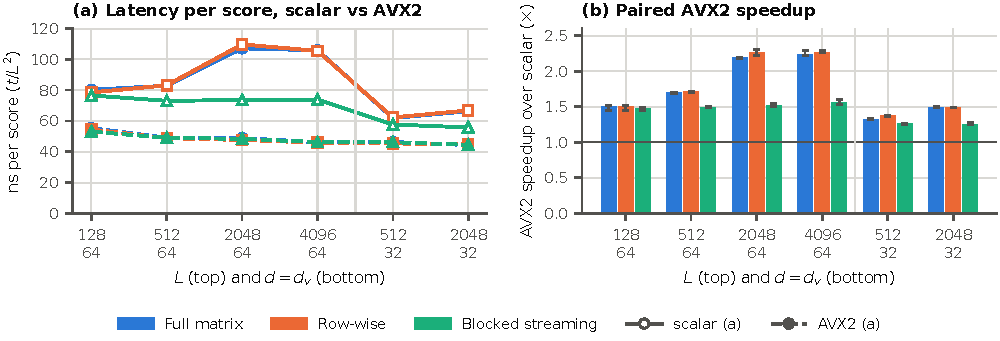
\includegraphics[width=\textwidth]{figures/fig_simd.pdf}
\caption{Single-thread results for the six shapes. (a) Median latency divided by $L^2$ (time per score); solid lines with open markers are scalar, dashed lines with filled markers are AVX2. (b) AVX2 speedup over scalar, formed within each batch; bars show the median and whiskers the range of the three batches.}
\label{fig:simd}
\end{figure}

\begin{table}[!htbp]
\centering\footnotesize
\caption{Single-thread latency in ms (median of batch medians) and paired AVX2 speedup over scalar.}
\label{tab:simd}
\setlength{\tabcolsep}{4pt}
\begin{tabular*}{\textwidth}{@{\extracolsep{\fill}}rr rrr rrr rrr@{}}
\toprule
& & \multicolumn{3}{c}{Scalar (ms)} & \multicolumn{3}{c}{AVX2 (ms)} & \multicolumn{3}{c}{AVX2 speedup ($\times$)}\\
\cmidrule(lr){3-5}\cmidrule(lr){6-8}\cmidrule(l){9-11}
$L$ & $d$ & full & row & blocked & full & row & blocked & full & row & blocked \\
\midrule
\inputtab generated/tab_simd.tex 
\bottomrule
\end{tabular*}
\end{table}

\subsection{Thread scaling}
At $L=4096$ two threads reach \gpn{t2min}--\gpn{t2max}$\times$ and four threads \gpn{t4min}--\gpn{t4max}$\times$ (efficiency \gpn{e4min}--\gpn{e4max}\%); eight threads drop to \gpn{t8min}--\gpn{t8max}$\times$ (\gpn{e8min}--\gpn{e8max}\%), so $T=8$ is \gpn{t8overt4-4096-min}--\gpn{t8overt4-4096-max}$\times$ slower than $T=4$ in all \gpn{t4wins-4096} route--batch pairs (Figure~\ref{fig:threads}, Table~\ref{tab:threads}). At $L=128$ four threads reach only \gpn{s128t4min}--\gpn{s128t4max}$\times$, and $T=4$ beats $T=8$ in \gpn{t4wins-128} of 9 route--batch pairs; in batch \gpn{t8excbatch} eight threads were faster for all three routes. The three routes scale almost identically.

\begin{figure}[!htbp]
\centering
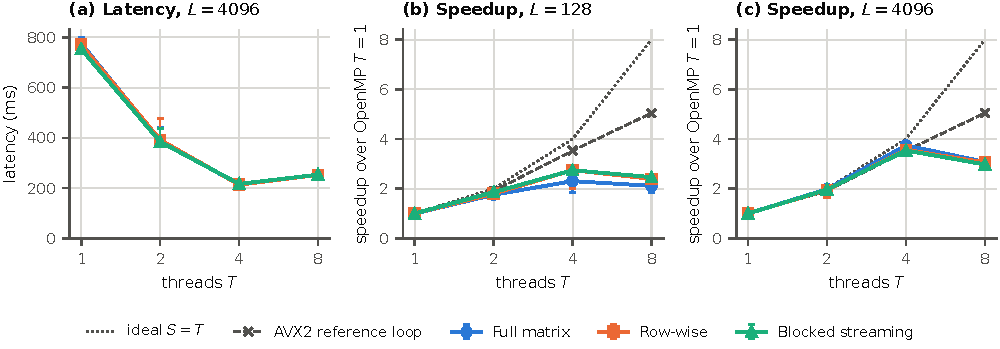
\includegraphics[width=\textwidth]{figures/fig_threads.pdf}
\caption{OpenMP scaling. (a) Latency at $L=4096$, $d=d_v=64$. (b, c) Speedup over the same route's OpenMP $T=1$ call within each batch at $L=128$ and $L=4096$. Points are medians of three batches; bars show the batch range. The dashed grey line is the speedup that an equal static split would get if each thread ran like the AVX2 reference loop on its CPU (Section~\ref{sec:threads}). $T=8$ includes four lower-class cores.}
\label{fig:threads}
\end{figure}

\begin{table}[!htbp]
\centering\footnotesize
\caption{OpenMP speedup over the same route at $T=1$ (median [min, max] of paired batch ratios) and parallel efficiency $S/T$ in percent. The last row is the AVX2 reference loop with fixed work per thread (time in ms).}
\label{tab:threads}
\setlength{\tabcolsep}{4pt}
\begin{tabular*}{\textwidth}{@{\extracolsep{\fill}}r l r lll rrr@{}}
\toprule
$L$ & Route & $T=1$ (ms) & $S(2)$ & $S(4)$ & $S(8)$ & $E(2)$ & $E(4)$ & $E(8)$ \\
\midrule
\inputtab generated/tab_threads.tex 
\bottomrule
\end{tabular*}
\end{table}

\subsection{Key-block tuning}
The three key-block sizes gave the same time within \gpn{tunespread}\% (Table~\ref{tab:tuning}). The same candidate varied by \gpn{tunebatchspread}\% between batches, and each batch had a different winner (\gpn{tunewinners}). The frozen rule picked $\Bk=\gpn{bk}$, which therefore reflects the rule, not a measurable optimum.

\begin{table}[!htbp]
\centering\footnotesize
\caption{Scalar blocked streaming at $L=2048$, $d=d_v=64$, $\Bq=16$: batch medians in ms. The selection value is the median of the three.}
\label{tab:tuning}
\begin{tabular}{@{}r r rrr r@{}}
\toprule
$\Bk$ & Workspace (bytes) & Batch 1 & Batch 2 & Batch 3 & Selection value \\
\midrule
\inputtab generated/tab_tuning.tex 
\bottomrule
\end{tabular}
\end{table}

\subsection{PyTorch CPU SDPA}\label{sec:torch}
PyTorch was faster in every configuration, by \gpn{ptratiomin}--\gpn{ptratiomax}$\times$ against our fastest route (Figure~\ref{fig:torch}, Table~\ref{tab:torch}). On one thread the gap is \gpn{ptratio-2048-T1}$\times$ at $L=2048$ and \gpn{ptratio-4096-T1}$\times$ at $L=4096$, and it is largest at $d=32$; it is smallest at $L=128$ with several threads, where both libraries spend much of the call on fixed costs. On one thread PyTorch reaches \gpn{ptgf-4096-T1}\,GFLOP/s of matrix work at $L=4096$, above our non-FMA reference loop (\gpn{calC-T1}\,GFLOP/s). Relative to the native harness, our routes change by \gpn{apinativemin}\% to \gpn{apinativemax}\% through the API at $L=4096$ on one thread, so the API scope does not change the comparison.

\begin{figure}[!htbp]
\centering
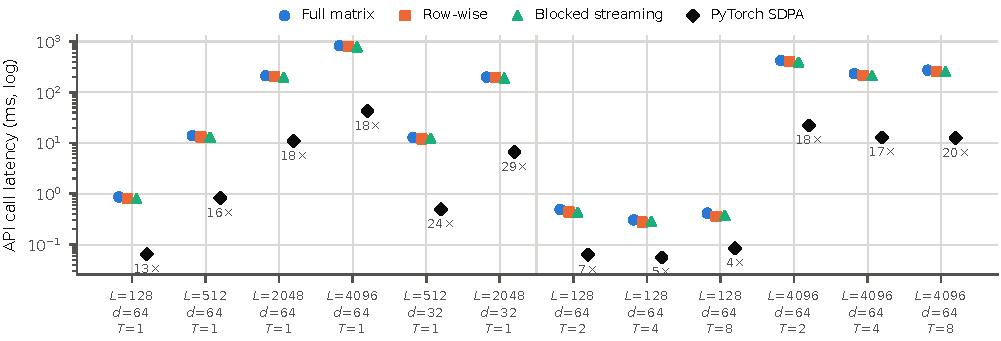
\includegraphics[width=\textwidth]{figures/fig_pytorch.pdf}
\caption{API-level latency (log scale) of our three routes and PyTorch SDPA, one batch of 20 calls each. Our routes use AVX2 at $T=1$ and AVX2\,+\,OpenMP at $T>1$. Labels give our fastest route's latency divided by PyTorch's.}
\label{fig:torch}
\end{figure}

\begin{table}[!htbp]
\centering\footnotesize
\caption{API-level median latency in ms (allocation and dispatch included) and the ratio of our fastest route to PyTorch.}
\label{tab:torch}
\begin{tabular}{@{}rrr rrr r r@{}}
\toprule
$L$ & $d$ & $T$ & full & row & blocked & PyTorch & ratio \\
\midrule
\inputtab generated/tab_pytorch.tex 
\bottomrule
\end{tabular}
\end{table}

\subsection{Variability}\label{sec:var}
Run-to-run noise is small for large shapes and large for small ones. The IQR exceeds 10\% of the median in \gpn{nvarten} of the \gpn{ninst} configuration instances and 20\% in \gpn{nvartwenty}; the worst case is \gpn{varmax}\% (\gpn{varmaxcfg}), while the median for $L\ge2048$ is \gpn{varmedbig}\%. Batch medians of the same serial configuration differ by a median of \gpn{bspreadmed}\% (up to \gpn{bspreadmax}\%), but paired AVX2/scalar ratios move by only \gpn{pairspreadmed}\% (up to \gpn{pairspreadmax}\%) between batches. We therefore draw conclusions from paired ratios and treat absolute differences smaller than the batch-to-batch spread as ties.

%======================================================================
\section{Analysis}\label{sec:analysis}

\subsection{Where the time goes: per-score work dominates the AVX2 kernels}\label{sec:where}
Most of the AVX2 run time is spent on work that is done once per score and does not depend on $d$. If the time of a variant is $t=L^2(a+b\,d)$ with $d=d_v$, the two head dimensions measured at the same $L$ give $a$ and $b$, and the share of $a$ at $d=64$ is $2/\rho-1$, where $\rho=t_{64}/t_{32}$. Table~\ref{tab:dscale} applies this to the paired data. For AVX2, $\rho$ is only \gpn{rhosimdmin}--\gpn{rhosimdmax}: doubling the matrix work barely changes the time, and \gpn{simdsharemin}--\gpn{simdsharemax}\% of it (\gpn{simdamin}--\gpn{simdamax}\,ns of \gpn{simdtotmin}--\gpn{simdtotmax}\,ns per score) belongs to the $d$-independent part.

\begin{table}[!htbp]
\centering\footnotesize
\caption{Effect of the head dimension at fixed $L$. $\rho=t(d{=}64)/t(d{=}32)$ (median of paired batch ratios); ns/score $=t(d{=}64)/L^2$; $a$ is the $d$-independent time per score and its share at $d=64$, from the affine model $t=L^2(a+bd)$.}
\label{tab:dscale}
\setlength{\tabcolsep}{4pt}
\begin{tabular*}{\textwidth}{@{\extracolsep{\fill}}l l rrrr rrrr@{}}
\toprule
& & \multicolumn{4}{c}{$L=512$} & \multicolumn{4}{c}{$L=2048$}\\
\cmidrule(lr){3-6}\cmidrule(l){7-10}
Mode & Route & $\rho$ & ns/score & $a$ (ns) & share & $\rho$ & ns/score & $a$ (ns) & share \\
\midrule
\inputtab generated/tab_dscale.tex 
\bottomrule
\end{tabular*}
\end{table}

The $d$-independent part is the same scalar code in both modes. Scalar blocked streaming, whose time also fits the affine model, shows $a=\gpn{ans-blk-scalar-512}$ and \gpn{ans-blk-scalar-2048}\,ns, the same as the AVX2 values. Per score this part contains one \code{expf} call through the double-precision x87 path, the maximum, sum and division passes of softmax, the scaling of the score and, in AVX2, the horizontal sum of the eight lanes. We did not time these pieces separately. The $d$-independent part is \gpn{aoverbmin}--\gpn{aoverbmax} times the time of the 128 multiplications and additions per score, and apart from the exponential each of its pieces is a few simple instructions, so the exponential is the most likely main cost.

\textbf{H3} holds in part: SIMD helps the inner products and softmax limits the gain, but memory traffic does not (Section~\ref{sec:roof}). Even if the matrix arithmetic became free, the AVX2 kernels could speed up by at most \gpn{amdmin}--\gpn{amdmax}$\times$; the next step must make the exponential cheaper (a vector exponential) or amortise it, not widen the dot product.

\subsection{Why scalar blocked streaming is faster: loop order, not workspace}\label{sec:loop}
In scalar mode, blocked streaming needs \gpn{blkgainmin}\% less time than row-wise at $L=128$ and \gpn{blkgain-scalar-4096-64}\% less at $L=4096$, while full-matrix and row-wise stay within \gpn{fullrowsc-dev}\% of each other at every shape (paired ratio \gpn{fullrowsc-min}--\gpn{fullrowsc-max}). Materialising the score matrix therefore costs nothing measurable here; the difference comes from the $PV$ loop.

The scalar full-matrix and row-wise kernels compute each output element as a sum down one column of $V$: a chain of $L$ dependent additions that reads one element from each $V$ row. One such sweep touches $L$ cache lines, i.e.\ \gpn{colws-512}\,KiB at $L=512$ and \gpn{colws-2048}\,KiB at $L=2048$ with 64-byte lines, and the next output element sweeps the same lines again. Blocked streaming instead adds $p_j v_j$ to $d_v$ independent accumulators, reading each $V$ row contiguously once per query block. Two observations support this explanation. First, the scalar full-matrix time per score jumps from about \gpn{totns-full-scalar-512} to \gpn{totns-full-scalar-2048}\,ns (row-wise: \gpn{totns-row-scalar-512} to \gpn{totns-row-scalar-2048}\,ns) between $L=512$ and $L=2048$, where the column sweep grows beyond the size of a typical first-level data cache, while blocked streaming stays at \gpn{totns-blk-scalar-512}--\gpn{totns-blk-scalar-2048}\,ns. Row-wise shows the same jump although it never stores $S$, so the score matrix is not the cause. Second, the same jump inflates the $d$-dependent part, so the affine model gives full and row-wise a smaller $a$ at $L=2048$ (Table~\ref{tab:dscale}). We did not count cache misses, so this remains an inference from timing.

The AVX2 versions of all three routes use the row order, which is why they converge. At $L=4096$ the per-score time falls from \gpn{pers-full-scalar-4096}\,ns (scalar full matrix) to \gpn{pers-blk-scalar-4096}\,ns (scalar blocked, row order) to \gpn{pers-full-simd-4096}\,ns (AVX2): about \gpn{loopfactor}$\times$ from loop order and \gpn{vecfactor}$\times$ from vector arithmetic. Part of the large AVX2 speedup of full-matrix and row-wise is therefore a loop interchange that the scalar baseline could also adopt.

\subsection{Memory traffic and the roofline view}\label{sec:roof}
Compared with full-matrix, streaming reduces the workspace by a factor of \gpn{wsratio} at $L=4096$ and the modelled DRAM traffic by \gpn{trafficratio}$\times$ (read-once scenario below), but none of the kernels is limited by memory bandwidth, so this reduction does not show up in time. We cannot measure DRAM bytes on this laptop, so Table~\ref{tab:roofline} uses two assumed scenarios per route: an optimistic one where $Q$, $K$ and $V$ are read once, and a pessimistic one where $K$ and $V$ are fetched again for every query (full, row-wise) or every query block (blocked). Both count output stores with read-for-ownership; the full-matrix route adds five passes over its \gpn{wsfullmib}\,MiB score matrix (write with read-for-ownership, read and write back in softmax, read in $PV$), which cannot stay in the \gpn{lthree}\,MiB L3. Even in the pessimistic case the bandwidth that the measured time implies is at most \gpn{bwpct-full-refill-T1}\% of the measured read rate on one core and \gpn{bwpct-full-refill-T4}\% on four; in the read-once case the full-matrix route needs \gpn{bw-full-once-T1}\,GB/s, \gpn{bwpct-full-once-T1}\% of what one core can read.

\begin{table}[!htbp]
\centering\footnotesize
\caption{Modelled DRAM traffic at $L=4096$, $d=d_v=64$ ($F_{\mathrm{mat}}=\gpn{Fmat}$\,GFLOP) and the bandwidth the measured AVX2 ($T=1$) and OpenMP ($T=4$) times would require, also as a share of the measured read-stream rate at the same $T$. Traffic is a model, not a measurement.}
\label{tab:roofline}
\setlength{\tabcolsep}{4pt}
\begin{tabular*}{\textwidth}{@{\extracolsep{\fill}}l l r r rr rr@{}}
\toprule
Route & Scenario & Modelled bytes & FLOP/byte & GB/s, $T=1$ & of read ref. & GB/s, $T=4$ & of read ref. \\
\midrule
\inputtab generated/tab_roofline.tex 
\bottomrule
\end{tabular*}
\end{table}

Figure~\ref{fig:roof} places the kernels on a roofline~\cite{williams2009} built from our two reference workloads. Whichever scenario applies, every point sits below both the bandwidth line and the compute line, and far below except in the pessimistic scenario on four threads, where full-matrix and row-wise would need \gpn{bwpct-row-refill-T4}--\gpn{bwpct-full-refill-T4}\% of the read rate: the AVX2 kernels reach \gpn{gf-full-T1}--\gpn{gf-row-T1}\,GFLOP/s on one core (\gpn{pctC-full-T1}\% of the reference loop) and \gpn{gf-blk-T4}--\gpn{gf-full-T4}\,GFLOP/s on four (\gpn{pctC-full-T4}\%). The roofline is a model of what could bound the kernel; here it rules out bandwidth as the limit and points back to the in-core per-score work of Section~\ref{sec:where}. PyTorch's single-thread throughput lies above our compute line, which shows that this line, measured without FMA, is a reference for our instruction mix rather than the peak of the core.

\begin{figure}[!htbp]
\centering
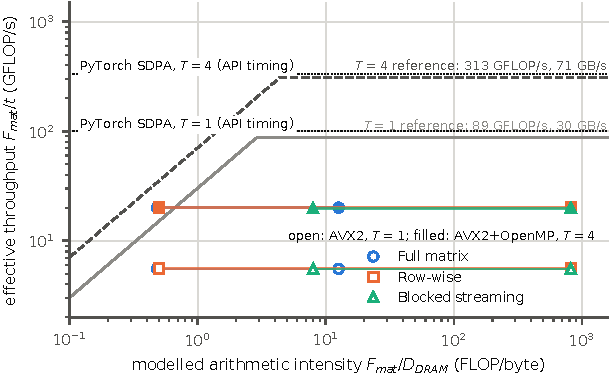
\includegraphics[width=0.66\textwidth]{figures/fig_roofline.pdf}
\caption{Roofline placement at $L=4096$, $d=d_v=64$. Solid and dashed lines: $\min(C,B\cdot I)$ from the measured AVX2 multiply--add rate $C$ and read-stream rate $B$ at $T=1$ and $T=4$. Each route appears twice at the same measured throughput, once per traffic scenario of Table~\ref{tab:roofline}; the segment joins the two. Dotted lines: PyTorch throughput at the same shape (API timing).}
\label{fig:roof}
\end{figure}

This answers \textbf{H1} in two parts. Streaming does reduce workspace and, under both traffic models, DRAM traffic. On this machine and up to $L=4096$ that reduction buys no time, because the kernels are compute-bound in the per-score work. Its real value at this scale is memory capacity: the full-matrix workspace grows as $L^2$ and the blocked one does not.

\subsection{Blocking and block size (H2)}\label{sec:h2}
The tuning data do not support \textbf{H2} within the range we tested. The three $\Bk$ values differ by \gpn{tunespread}\%, well inside the batch-to-batch spread, and no cache-driven optimum appears. This fits Section~\ref{sec:where}: $\Bk$ changes only the tile working set and how often the state is rescaled (one rescale of $d_v$ values and one extra exponential per query row and key block, i.e.\ about \gpn{rescalepct}\% extra work at $\Bk=128$), while most of the time goes to per-score work that $\Bk$ does not touch. A cache effect might appear with much larger tiles, with $\Bq$ tuning, or once the exponential is cheap; we did not test these.

\subsection{Thread scaling (H4)}\label{sec:threads}
\textbf{H4} holds: at $T=4$ the large input scales to \gpn{t4min}--\gpn{t4max}$\times$ and the small one only to \gpn{s128t4min}--\gpn{s128t4max}$\times$. Three effects explain the shape of Figure~\ref{fig:threads}.

\emph{Up to four threads, the loss tracks the clock of the busy cores.} The reference loop does fixed work per thread, so its time at $T$ threads shows how fast each core runs when $T$ cores are busy. It slows by \gpn{calslow-T2}\% at $T=2$ and \gpn{calslow-T4}\% at $T=4$, giving an expected speedup of \gpn{calspeed-T2} and \gpn{calspeed-T4}; the attention kernels at $L=4096$ reach \gpn{t2min}--\gpn{t2max} and \gpn{t4min}--\gpn{t4max}. A lower clock with more active cores is the likely cause, but we did not record frequency.

\emph{At eight threads, the static split waits for the slowest core.} With $L=4096$ and $\Bq=16$ there are \gpn{nblk-4096} query blocks, so each of eight threads gets \gpn{nblkthr-4096}. Four of those threads run on CPU4--7, which Windows places in the lower efficiency class. With equal shares, an efficiency of \gpn{e8min}--\gpn{e8max}\% means that the slowest thread processed its share \gpn{slowfactor8min}--\gpn{slowfactor8max}$\times$ slower than CPU0 alone would. The reference loop shows a smaller factor (\gpn{calslowfactor8}$\times$) for pure multiply--add work, so the attention instruction mix, likely the x87 exponential, runs relatively worse on those cores; we did not record per-thread times to confirm this. Dynamic scheduling or a split weighted by core class targets this loss directly; we did not test either. On this laptop $T=4$ is the best setting.

\emph{At $L=128$, fixed parallel costs dominate.} There are only \gpn{nblk-128} query blocks of work worth \gpn{t1-128-min}--\gpn{t1-128-max}\,$\mu$s on one thread. Writing $t_T=t_1/T+c$ for $T\in\{2,4\}$ gives a fixed cost $c$ of \gpn{ovhmed}\,$\mu$s (median; range \gpn{ovhmin}--\gpn{ovhmax}\,$\mu$s), which includes waking passive workers, scheduling and the barriers. The noisiest configurations in the study are these small multi-threaded ones. At one thread the OpenMP call was as fast as the serial AVX2 call or faster, within noise (\gpn{omp1oversimd-4096-min}\% to \gpn{omp1oversimd-4096-max}\% at $L=4096$; \gpn{omp1oversimd-128-min}\% to \gpn{omp1oversimd-128-max}\% at $L=128$, a cross-process difference of the size of the batch spread), so the parallel region adds no measurable cost when no worker must be woken.

\subsection{What PyTorch does differently}
PyTorch's whole call costs \gpn{ptpers-4096}\,ns per score at $L=4096$ on one thread, about \gpn{ptpersratio} times less than the $d$-independent part alone in our AVX2 kernels (at least \gpn{simdamin}\,ns per score, measured at $L=512$ and $2048$). The profiler names the selected operator \texttt{\gpn{torchop}}; going by that name it is a FlashAttention-style kernel~\cite{dao2022}, that is, also a tiled computation with an online softmax. We did not read its source. If the name is accurate, the gap does not come from the route; it comes from how a tile is computed. Its \gpn{ptgf-4096-T1}\,GFLOP/s on one core exceeds our reference loop, so its matrix kernels run closer to the core's peak than any of our code; and since its whole cost per score is only \gpn{ptpers-4096}\,ns, its exponential must be far cheaper than our scalar x87 path. These are the two optional extensions in the proposal (a packed microkernel and a fast exponential) that we did not attempt. PyTorch also scales only \gpn{ptspeed-4096-T4}$\times$ from one to four threads and \gpn{ptspeed-4096-T8}$\times$ to eight, so it meets the same limits on this hybrid CPU.

\subsection{When each route is beneficial}
\begin{itemize}
\item \textbf{Full matrix} is never faster by more than noise in our measurements: where its median is the lowest (AVX2 at $L=2048$, $d=32$; eight threads at $L=4096$) the margin over the next route is about \gpn{fullbestmargin}\% or less. Its cost is memory capacity: \gpn{wsfullmib}\,MiB at $L=4096$, growing as $L^2$.
\item \textbf{Row-wise} matches the full-matrix time with $L/\Bq$ times less workspace, so it is the better of the two whenever the full $P$ matrix is not needed as an output.
\item \textbf{Blocked streaming} uses a workspace independent of $L$ (\gpn{ws-blk-4096}\,bytes), is the fastest scalar route for $L\ge512$, and ties the others with AVX2. It is the best default, and it is the only route whose structure leaves room for the next optimisations (register-blocked tiles and a vector exponential applied per tile).
\item \textbf{Threads} pay off most for large $L$; on this hybrid CPU four threads on the high-performance cores beat eight threads with a static split.
\end{itemize}

%======================================================================
\section{Limitations and proposal coverage}\label{sec:limits}

\textbf{Measurement limits.} All timings come from one laptop. Clock frequency and temperature were not fixed or logged, and affinity was a process mask, not per-thread pinning. We had no hardware counters, so DRAM traffic and cache behaviour are modelled or inferred from timing, and the share of the exponential is inferred from the head-dimension model rather than profiled. The PyTorch comparison has a single batch and two different OpenMP runtimes. Small multi-threaded shapes are noisy (Section~\ref{sec:var}).

\textbf{Implementation limits.} The AVX2 dot product uses one accumulator and sums lanes for every score; there is no FMA, no register blocking, no packing and no vector exponential. Only $\Bk$ was tuned, only in scalar mode, and the same $\Bk$ was used for every mode. The OpenMP schedule is static and ignores core classes.

\textbf{Code version.} The timings belong to revision \code{\gpn{srcrev}}. The later commits on the submitted branch add workspace-size overflow checks for the row-wise helper and change documentation, analysis scripts and tests; no timed kernel changed. All suites were re-run on the later revision.

\begin{table}[!htbp]
\centering\small
\caption{Proposal items and their status.}
\label{tab:coverage}
\begin{tabularx}{\textwidth}{@{}Y l Y@{}}
\toprule
Proposal item & Status & Where / note \\
\midrule
Three routes $\times$ scalar, SIMD, SIMD + static OpenMP; FP64 oracle; boundary tests & done & Sections~\ref{sec:impl}, \ref{sec:correct} \\
Six-shape scalar/SIMD grid; 3$\times$3 tables at $L=128$, $4096$; thread counts $\{1,2,4,8\}$ & done & Tables~\ref{tab:main}--\ref{tab:threads} \\
$\Bq=16$, $\Bk$ scan frozen before main runs & done & Table~\ref{tab:tuning}; only scalar, only $\Bk$ \\
Median, variation, throughput, error, workspace & done & Section~\ref{sec:results} \\
SIMD evidence (compiler report or assembly) & done & disassembly of the measured binary \\
Record FMA/reduction choices, alignment, affinity & done & Section~\ref{sec:impl}, Table~\ref{tab:setup}; alignment not controlled (unaligned loads) \\
Bandwidth measurement and roofline model (target) & done & Section~\ref{sec:roof}; read bandwidth measured, kernel traffic modelled, not measured \\
PyTorch CPU SDPA comparison with recorded backend (target) & done & Section~\ref{sec:torch}; one batch \\
Counter-based traffic measurement & not done & no hardware counters available \\
Optional extension: packed microkernel or fast exponential & not done & not attempted; Section~\ref{sec:analysis} shows where it would help \\
Reproduce frozen results (Week 6) & partly & fresh clone rebuilt, all suites pass; archived statistics recomputed from raw samples with no disagreement; timings not re-measured \\
\bottomrule
\end{tabularx}
\end{table}

%======================================================================
\section{Reproduction}\label{sec:repro}

The repository (\url{https://github.com/szwww2/ATTENTION_OPTIMIZATION_on_CPU}) contains the sources, the seven C++ suites, the Python tests, all runners and analysis scripts, and the archived study in \code{examples/controlled\_20261023/} with SHA-256 sums for every file. The work was integrated on branch \code{dev/chencaoyu-integration} (pull request \#5); the assessed version is \showversion. Requirements: GCC with OpenMP on an AVX2 CPU, Python~3 with NumPy and Matplotlib; PyTorch \gpn{torchver} (CPU build) only for the API comparison. From the repository root:

{\footnotesize
\begin{verbatim}
python tools/build_integrated.py          # nine variants, benchmark and seven test programs
build/attn_tests       build/attn_blocks        build/attn_simd_kernels_tests
build/attn_simd_tests  build/attn_omp_tests     build/attn_streaming_tests
build/attn_streaming_optimized_tests            # add .exe on Windows
python tests/test_nine_mode_benchmark.py
python tools/run_scalar_bench.py --suite optimized --streaming --key-block 128 --mode all \
    --threads 2 --L 128 --query-block 16 --warmup 1 --reps 3 --out results/nine_check
python examples/controlled_20261023/verify_package.py    # integrity of the archived study
python report/make_numbers.py                            # every number, table and figure here
\end{verbatim}}

\code{make\_numbers.py} recomputes all statistics in this report from the raw samples and compares them with the archived summary tables (\gpn{ninst} instances; no disagreement). A new full study needs the same kind of machine and a clean committed tree:

{\footnotesize
\begin{verbatim}
set OMP_WAIT_POLICY=PASSIVE                     # Linux: export OMP_WAIT_POLICY=PASSIVE
python tools/run_controlled_study.py --out results/my_study --physical-cores 16 \
    --cpu-order 0,1,2,3,4,5,6,7
python tools/run_pytorch_grid.py --physical-cores 16 --cpu-order 0,1,2,3,4,5,6,7 \
    --frozen-settings results/my_study/frozen_settings.json --out results/my_study/pytorch
python tools/run_roofline_calibration.py --out results/my_calibration --cpu-order 0,1,2,3,4,5,6,7
\end{verbatim}}
The CPU order must list the high-performance cores first on the machine in use. Absolute times will differ on other machines; the paired ratios are the quantities to compare.

%======================================================================
\section{Member contributions}\label{sec:contrib}

Table~\ref{tab:contrib} summarises each member's work as recorded in the repository\ifallconfirmed{; every member has checked and confirmed their own row.}{. Each member confirms their own row.}

\begin{table}[!htbp]
\centering\small
\caption{Member contributions.}
\label{tab:contrib}
\ifallconfirmed{\begin{tabularx}{\textwidth}{@{}l Y@{}}}{\begin{tabularx}{\textwidth}{@{}l Y l@{}}}
\toprule
Member & Contribution \ifallconfirmed{}{& Confirmed} \\
\midrule
Li Ruiqin & Initial repository layout and shared interface; deterministic input generator; independent FP64 oracle and error metric; scalar full-matrix and row-wise baselines; contract and block-size test suites with the boundary cases; NumPy cross-check; first timing loop; environment and PyTorch availability notes; Week~1 notes \confcell{Li}{Li Ruiqin} \\
Cui Ziwei & Blocked streaming with online softmax in scalar, AVX2 and OpenMP form; workspace sizing and argument checks; the two streaming test suites (tile sizes, key-block permutations, rescaling case, guards, concurrency); first tile-size pilot and streaming documentation; repository owner, merged PR~\#6 \confcell{Cui}{Cui Ziwei} \\
Tang Zhenxiong & Shared AVX2 dot-product and weighted-add helpers; AVX2 and OpenMP versions of full-matrix and row-wise; SIMD, helper and OpenMP test suites; CPU-topology tool; exploratory MSVC measurements and assembly evidence on his machine (not used for final numbers) \confcell{Tang}{Tang Zhenxiong} \\
Chen Caoyu & Validated benchmark harness and its gates; three-phase full-matrix fix; integration of all nine variants; integrated build; controlled-study runner, tuning and freezing; the final study; analysis and plotting tools; PyTorch bridge and comparison; roofline calibration and traffic model; code-generation evidence; reproduction guide; the first version of this report (with Claude, Section~\ref{sec:ai}) \confcell{Chen}{Chen Caoyu} \\
\bottomrule
\end{tabularx}
\end{table}


%======================================================================
\section{AI-use declaration}\label{sec:ai}

Each member declares their own use of AI tools.

\textbf{Chen Caoyu.} \showai{Chen}

\textbf{Cui Ziwei.} \showai{Cui}

\textbf{Li Ruiqin.} \showai{Li}

\textbf{Tang Zhenxiong.} \showai{Tang}

%======================================================================
\begin{thebibliography}{9}\small
\setlength{\itemsep}{1pt}
\bibitem{vaswani2017} A.~Vaswani, N.~Shazeer, N.~Parmar, J.~Uszkoreit, L.~Jones, A.~N.~Gomez, {\L}.~Kaiser and I.~Polosukhin, ``Attention is all you need,'' in \emph{Advances in Neural Information Processing Systems 30 (NeurIPS)}, 2017.
\bibitem{milakov2018} M.~Milakov and N.~Gimelshein, ``Online normalizer calculation for softmax,'' arXiv:1805.02867, 2018.
\bibitem{dao2022} T.~Dao, D.~Y.~Fu, S.~Ermon, A.~Rudra and C.~R{\'e}, ``FlashAttention: Fast and memory-efficient exact attention with IO-awareness,'' in \emph{Advances in Neural Information Processing Systems 35 (NeurIPS)}, 2022.
\bibitem{williams2009} S.~Williams, A.~Waterman and D.~Patterson, ``Roofline: An insightful visual performance model for multicore architectures,'' \emph{Communications of the ACM}, vol.~52, no.~4, pp.~65--76, 2009.
\bibitem{steele2014} G.~L.~Steele Jr., D.~Lea and C.~H.~Flood, ``Fast splittable pseudorandom number generators,'' in \emph{Proc.\ ACM OOPSLA}, pp.~453--472, 2014.
\bibitem{openmp52} OpenMP Architecture Review Board, \emph{OpenMP Application Programming Interface}, Version~5.2, November 2021.
\bibitem{pytorchsdpa} PyTorch documentation, ``torch.nn.functional.scaled\_dot\_product\_attention,'' \url{https://docs.pytorch.org/docs/stable/generated/torch.nn.functional.scaled_dot_product_attention.html}.
\end{thebibliography}

\end{document}
